% Chapter 2

\chapter{The LHC and CMS experiment} % 
\section{The Large Hardon Collider}
%LHC intro 
The LHC is a 27km circular circumference storage ring, accelerator and collider for 
both protons and Pb ions. It is situated in a stable environment in a tunnel 
100 metres underneath the Franco-Swiss boder near Geneva, Switzerland.
A double-ring synchotron, it is designed to collide proton-proton (pp)
pairs with a centre of mass energy of up to $\sqrt(s)=14\TeV$ and a 
luminosity of up to $10^{34}cm^{-2}s^{-1}$. This makes the LHC the only collider
in operation able to directly probe the $\TeV$ scale physics. 

The injected beams in the LHC are accelerated and stored for each physics run using 
a $400MHz$ superconducting cavity system. The beams of protons or pB ions 
are merged at four sections around the ring to enable collisions at interaction points.
At each of these four interaction points lies one of the four main 
experiments at the LHC; A Large Ion Collidor Experiment (ALICE) \cite{ALICE},
A Toroidal LHC Apparatus (ATLAS) \cite{ATLAS}, the Compact Muon solinoid (CMS) \cite{CMS}
and LHCb which record the collisions. Figure~\ref{} shows the layout of the LHC ring including
the positions of the four main detectors. The proton beams are made up of many 'bunches' of approximately $1.1\times10^{11}$
protons localised into less than 1 ns in the direction of motion.
The beams are formed inside the Proton Synchrotron (PS) from bunches of protons 25 or 50 ns apart with an energy of 26 GeV. 
The protons are then accelerated in the Super Proton Synchrotron (SPS) to 450 GeV before being injected into the LHC at
the points shown in Figure~\ref{}. Once injected into the LHC, Radio Frequency (RF) cavities 
provide around 275kW of RF power independently to each beam to accelerate the protons to allow collisions
at the operating centre of mass energy. For the work contained in the thesis $\sqrt(s) = 13\TeV$ with bunch spacings of both
25ns and 50 ns \cite{LHC}. The LHC operates as a storage ring for the accelerated beams using 1232 
superconducting dipole magnets in the eight arc segments which provide magnetic fields of up to $8T$ to steer the beams. 
High precision quadropole and higher order magnets at the interacton points are used to position and focus the beams to 
maximise the occurance of high momentum pp collisions. The average number of simultaneous collisions
per bunch crossing, in time pile-up (PU), for the work in this thesis was $\approx25$.
The luminosity in the LHC is not constant over a physics run, but decays due to the degradation 
of intensities and emittances of the circulating beams (mainly due to loss from collisions). Eventually,
the beam is dumped and the acceleration process is started again. The turn around time between dumping
the beam and the start of a new physics run is typically around 6 hours.

%%%FIGURE - LHC diagram!

\subsection{LHC run condictions}

The first physics runs of the LHC from 2010-2013 (Run 1) reached energies of 3.5 and 4 TeV per beam and 
provided record-breaking integrated luminosities. The data collected allowed 
for the discovery of the higgs boson\cite{higgs} as well as enabling many new regions of parameter space
to be probed. From 2013 to mid-2015 (Long Shutdown 1) the LHC was shut down for upgrade to allow design
energies to be reached. All magnet interconnectors were inspected and replaced where necessary 
and the dipole magnets underwent a quench training programme. 

After LS1, from 2015-2016 (Run 2, which will continue up to 2018) the LHC has been running with record beam energies 
of $6.5\TeV$ per beam with bunch spacings of 25 and 50 ns. 
As shown in Figure **, as of XX, the CMS and ATLAS detectors have been able to collect XX $fb^{-1}$ of integrated luminosity. 
This has enabled large areas of parameter space to be probed and limits to be set on new physics models. It is this 
XX/fb dataset, at a centre of mass energy of $\sqrt(s) = 13\TeV$, which is used in Chapters XX to search for Supersymmetry at the highest energy reached at a collider.

%%%FIGURE - LHC lumi plot!

%----------------------------------------------------------------------------------------
\section{The CMS detector}
The Compact Muon Solenoid (CMS \cite{CMSTDR}) is one of two general purpose detectors at the LHC 
which have performed exceptionally well during run 1. It is described in detail in \cite{CMS}. 

\begin{figure}
\centering
    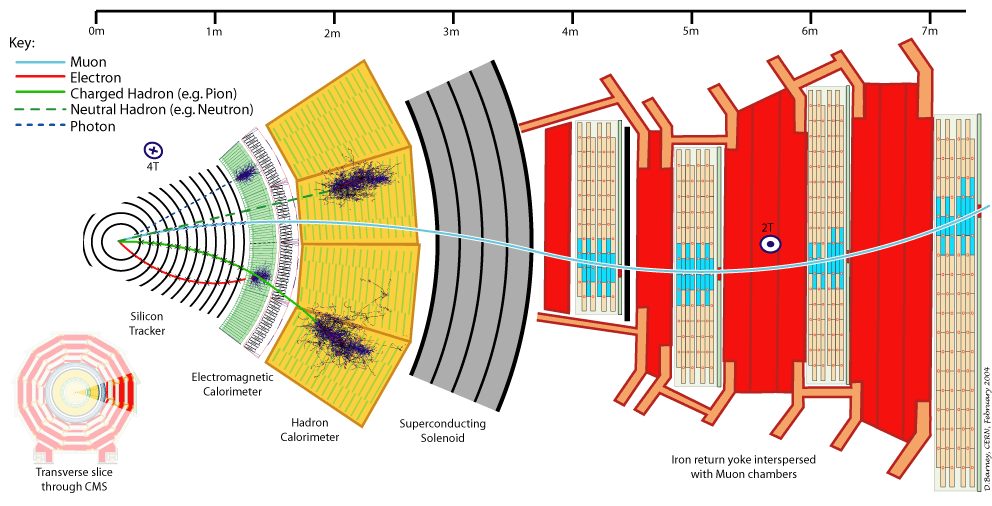
\includegraphics[width=0.9\textwidth]{./Figures/CMS_Slice.jpg}
  \caption{Cross Section of CMS showing the paths of various particle types 
  through different segments of the detector \cite{cmsslice}}
  \label{CMS_SLICE}
\end{figure}

A cross section of CMS is shown in figure \ref{CMS_SLICE}. The coordinate system used by CMS takes the origin at 
the collision point. The z-axis points along the beam direction and defines the azimuthal angle, $\phi$. 
Instead of the polar angle, $\theta$, the psuedorapidity, $\eta=-ln(tan(\theta/2))$, is used as $\Delta \eta$
between two particles is approximately relativistically invariant. The eta coverage of CMS is $|\eta|<5$. 
Transverse energies and momenta ($E_T $ and $p_T$)  are defined perpendicular to the beam \cite{cmsiop}. 
The different detector components shown in figure \ref{CMS_SLICE} will now be described in detail. 
Resolutions are quoted for measuring the relevant property for a 100 GeV particle/jet \cite{SACharacteristics}.
\begin{description}
\item[Silicon Tracker]The job of the tracker is to measure the momentum of charged particles from their path through a magnetic field \cite{siliconTDR}. The CMS tracker achieves $10\mu m$ accuracy with coverage for $|\eta|<2.5$ and has a resolution of 1\%.
\item[Electromagnetic Calorimeter (ECAL)] The ECAL measures the energy of incident photons and electrons. The ECAL barrel is made of 61,200 $PbWO_4$ crystals and provides coverage for $|\eta|<1.48$ \cite{ecal}. This is extended to $|\eta|<3$ by the endcap which adds another $10764$ crystals. The endcap has a pre-shower to distinguish between $\gamma$ and $\pi^0$. The ECAL has a resolution of 0.5\%.
 \item[Hadronic Calorimeter (HCAL)] The HCAL is made from alternating brass and scintilator layers with a coverage of $|\eta|<3.0$ \cite{hcal}. The coverage is extended to  $|\eta|<5.0$ by an iron/quartz forward calorimeter \cite{hfhcal}. The average resolution is 11\%. 
 \item[Muon Chambers]The muons are not stopped by any of the calorimeters and therefore require a separate detector with coverage $|\eta| < 2.4$. The muon chambers are interspersed with the magnet return yoke. The high magnetic field allows for accurate momentum measurement \cite{muons}. The resolution is 1\%.
\end{description}
As the data rate ($40Mhz$) is far too high for every event to be stored and as new physics will only 
be seen in a minority of events a trigger system for interesting events is necessary. 
This happens in two stages: the L1 Calorimetric and Muon Trigger (Hardware) and the High Level Trigger (Software) \cite{HLT}. 
The L1 trigger must operate within $\mathcal{O}10ns$ and so  the calorimetric trigger only takes input
from the ECAL and HCAL. This is described in more detail in chapter \ref{Chapter3}. The input from the
L1 triggers is then combined in the Global Trigger (GT) which decides whether to keep the event. 
The $\mathcal{O}100kHz$ events which pass L1 selection are processed in the HLT which utilises the 
calorimeter information along with tracking and the muon system to further reduce the rate to $\mathcal{O}1kHz$.
